\documentclass[11pt, a4paper]{exam}
\usepackage[utf8]{inputenc}
\usepackage{amsmath}
\usepackage{siunitx}
\usepackage{fixltx2e}
\usepackage{tikz}
\usetikzlibrary{decorations.pathreplacing}

\begin{document}
	\begin{questions}
		\question
		Assume that a Cepheid Variable, is the brightest when it is the most shrunk (radius $R_1$), and the faintest when it is the most expanded (radius $R_2$). Also assume that during this cycle, the star preserves its spherical shape and that it is a perfect black body. During its period of pulsation; the star's apparent magnitude varies between 3.46 and 4.08, and the wavelength at which its radiation peaks varies between \SI{531.0}{nm} and \SI{649.1}{nm}.
		\begin{parts}
			\part
			Find the ratio $\dfrac{R_1}{R_2}$ for the star.
			\part
			Find the radiation flux ($F_2$) of the star when it is the most expanded ($R_2$ = \SI{4.95e10}{\meter}).
			\part
			Find the distance of the star in parsecs.
		\end{parts}
		
		\question
		In a spectrographically observed galaxy cluster, the velocity dispersion of the member galaxies in a 1 Mpc radius has been determined as $\sigma =$ 750 km s$^{-1}$. Assuming that the mass found using the Virial Theorem represents the total mass of the cluester and that the average member galaxy has a mass of  \SI{e11}{M_\odot}, find the approximate number of galaxies in this galaxy cluster.
		
		\question
		The orbits of comets are usually very flattened, with eccentricities nearing 1, even exceeding 1 (hyperbolical orbits). Halley's comet has last approached Earth in the year 1986, its orbital period is $P$  = 76 yr and its eccentricity is $e = 0.9673$.
		\begin{parts}
			\part 
			What is the semi-major axis of the Halley's comet.
			\part 
			Approximate the mass of the Sun, assuming that the comet's only gravitational interaction is with the Sun.
			\part
			Find the distance between Halley's comet and the Sun, at perihelion and aphelion.
			\part
			The conjunction period of Venus is $S$ = 584 days. Using this information, compare the perihelion distances of Halley's comet and Venus; which is closer? Assume that the orbit of Venus is circular ($e = 0.007 \approx 0$)
		\end{parts}
		
		\question
		The CMB photons which were emitted when the universe was approximately 380000 years old are now detected as a black body with the temperature of 2.7K. In a state where CMB photons can be observed in the near infrared region with a K filter (central wevelength: 22000 \AA), what is the ratio between the size of the universe today and in that state?
		
		\question
		Let us have a thin and homogenous rod with mass $M = 36m$ and length $L$. The rod has been hung on its `O' end, such that it can freely rotate around that point. The rod is initially at rest.
		
		An object of mass $m$, with negligable volume, collides with and sticks to the vertical center of this rod ($L/2$ lower from the point `O'), with a velocity of $v_0 = \sqrt{37gL}$ parallel to the horizontal plane. The object and the rod together start to rotate around the pivot `O' and rise.
		
		If the rods moment of inertia with respect to the vertical passing from the point `O' is $I = \frac{1}{3}ML^2$, calculate the maximum height $h$ which the other end of the rod (point $B$) will have risen from its initial position.
		
		\question
		A white dwarf with mass \SI{1.34}{M_\odot}, is in a binary stellar system and \SI{4e7}{M_\odot} is transferred form the component star to its  surface every year.
		\begin{parts}
			\part
			If the rate of the transfer of mass stays constant, in how many years will the white dwarf's mass reach Chandrasekhar's Limit?
			
			\part
			Why does a Type I supernova (carbon explosion) occur when the white dwarf reaches the limit mass?
			
			\part
			\%90 of the total energy of the supernova is radiated in an isotropical (equal to every direction) and balanced manner in the first 25 days. If this first bright stage of the explosion's observed flux from the Earth is detected as \SI{5e-11}{\joule \meter^{-2} \second^{-1}}, calculate the distance of the exploding white dwarf from Earth in light years.
		\end{parts}
		
		\question
		Using the table given below;
		\begin{figure}[hbt!]
			\hspace{15pt}
			\begin{tabular}{c c c}
				\hline
				No & P ($\mu$ s) & a (m s$^{-2}$) \\
				\hline 
				1 & 7587.8889 & -0.92$\pm$0.08 \\
				2 & 7588.4100 & -1.68$\pm$0.04 \\
				3 & 7588.5810 & -1.67$\pm$0.06 \\
				4 & 7587.8836 & +0.72$\pm$0.06 \\
				5 & 7589.1029 & +0.52$\pm$0.08 \\
				6 & 7589.1350 & +0.00$\pm$0.04 \\
				7 & 7588.9800 & -1.04$\pm$0.02 \\ [1ex]
				\hline
			\end{tabular}
			\hspace{10pt}
			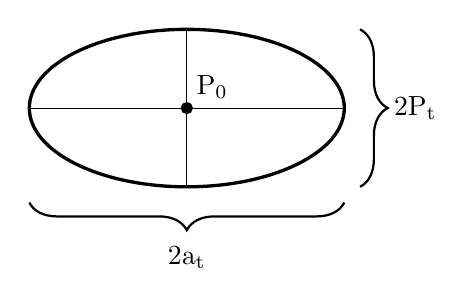
\begin{tikzpicture}[baseline=-3em]
				\draw (0,0) ellipse (2cm and 1cm)[very thick];
				\draw[-] (-2,0) -- (2,0);
				\draw[-] (0,-1) -- (0,1);
				\draw[fill] circle (2pt) node[above right] {P\textsubscript{0}};
				\draw[decorate, decoration={brace, amplitude=10pt, mirror}, thick] (-2,-1.2) -- (2,-1.2) node[midway,yshift=-2em] {2a\textsubscript{t}};
				\draw[decorate, decoration={brace, amplitude=10pt, mirror}, thick] (2.2,-1) -- (2.2,1) node[midway,xshift=2em] {2P\textsubscript{t}};
			\end{tikzpicture}
		\end{figure}
		\begin{parts}
			\part
			Sketch a $P-a$ graph on a millimetric graphing paper, add the error bars for the values of $a$, state the scaling you have used on the paper.
			
			\part
			Sketch the ellipse which best represents the points on the $P-a$ graph.
			
			\part
			Measure the values given on the ellipse above using a ruler. The errors of the values measured are given so: $\Delta P_0 = 0.02$, $\Delta a_0 = 0.06$, $\Delta P_t = 0.02$.
			
			\part
			Using the equation $P_B = P_t / P_0 \times 2 \pi c / a_t$, calculate $P_B$ and its uncertainty in days. Consider the rules of the propagation of uncertainty in your calculations. 
		\end{parts}
		
		\question
		Epsilon Lyrae ($\epsilon$ Lyr) with a distance of 162 ly from Earth, is a double-double star system located in the Lyra constellation. It was first identified as a binary star system and its components were designated $\epsilon^1$ and $\epsilon^2$. When observed with a telescope with higher angular resolution, it was seen that they each had two components with $\epsilon^1$'s being A and B, and $\epsilon^2$'s being C and D. The apparent magnitudes of these stars are A: 5.15, B: 6.10, C: 5.25 and D: 5.38. The angular distances of these components are given in the table.
		
		Let us consider the telescope that has been used in the Summer Camp observations; $f$ = 2000mm, Focal Ratio = $f/10$, $f$\textsubscript{ocular} = 25mm, FOV\textsubscript{ocular} = 60$^\circ$.
		
		\vspace{5pt}
		\begin{tabular}{c c c c}
			\hline
			Components & Distance ($^{\prime\prime}$) & Distance (au) & Notation \\
			\hline
			AB-CD & 208.2 & 10500 & $\epsilon^1$-$\epsilon^2$ \\
			AB & 2.3 & 116 & $\epsilon^1$ \\
			CD & 2.4 & 121 & $\epsilon^2$ \\ [1ex]
			\hline
		\end{tabular}
		\vspace{5pt}
		
		\begin{parts}
			\part
			In accordance with the information given in the table, if we were to observe the $\epsilon$ Lyr system with the telescope whose properties have been given, find through calculations the components which we would have been able to distinguish. Assume the visual wavelength to be 550 nm.
			
			\part
			What would be the optical minimum diameter of a telescope which would be able to distinguish all components of the system, in centimeters?
		\end{parts} 
	\end{questions}
\end{document}